\documentclass{article}

%\PassOptionsToPackage{numbers}{natbib}

%\usepackage{neurips_2019}
\usepackage{iclr2020_conference,times}

\usepackage[utf8]{inputenc} % allow utf-8 input
\usepackage[T1]{fontenc}    % use 8-bit T1 fonts
\usepackage[pdfborder={0 0 0}]{hyperref}       % hyperlinks
\usepackage{url}            % simple URL typesetting
\usepackage{booktabs}       % professional-quality tables
\usepackage{amsfonts}       % blackboard math symbols
\usepackage{nicefrac}       % compact symbols for 1/2, etc.
\usepackage{microtype}      % microtypography

\usepackage{subcaption}
\usepackage{graphicx}
\usepackage{amsmath}
\usepackage{amssymb}
\usepackage{bm}
\usepackage{relsize}
\usepackage{natbib}
\usepackage{float}
\usepackage{tikz}

\usetikzlibrary{shapes,arrows}

\tikzstyle{block} = [rectangle, draw, thick, align=center, rounded corners]
\tikzstyle{boundingbox} = [thick, lightgray]
\tikzstyle{dashblock} = [rectangle, draw, thick, align=center, dashed]
\tikzstyle{conc} = [ellipse, draw, thick, dashed, align=center]
\tikzstyle{netnode} = [circle, draw, very thick, inner sep=0pt, minimum size=0.5cm]
\tikzstyle{relunode} = [rectangle, draw, very thick, inner sep=0pt, minimum size=0.5cm]
\tikzstyle{line} = [draw, very thick, -latex']
\tikzstyle{arrow} = [draw, ->, thick]

\definecolor{bpurp}{HTML}{984ea3}
\definecolor{bblue}{HTML}{377eb8}

\setlength{\parskip}{1em}
\setlength{\parindent}{0em}

%\setcitestyle{square}

%\iclrfinalcopy % Uncomment for camera-ready version, but NOT for submission.
\begin{document}
\title{Zero-shot task adaptation by homoiconic meta-mapping}
\author{%
Andrew K. Lampinen\\
Department of Psychology\\
Stanford University\\
\texttt{lampinen@stanford.edu}\\
\And
James L. McClelland\\
Department of Psychology\\
Stanford University\\
\texttt{mcclelland@stanford.edu}\\
}
\date{}
\maketitle

\begin{abstract}
How can deep learning systems flexibly reuse their knowledge? Toward this goal, we propose a new class of challenges, and a class of architectures that can solve them. The challenges are meta-mappings, which involve systematically transforming task behaviors to adapt to new tasks zero-shot. We suggest that the key to achieving these challenges is representing the task being performed along with the computations used to perform it. We therefore draw inspiration from functional programming and recent work in meta-learning to propose a class of Homoiconic Meta-Mapping (HoMM) approaches that represent data points and tasks in a shared latent space, and learn to infer transformations of that space. HoMM approaches can be applied to any type of machine learning task, including supervised learning and reinforcement learning. We demonstrate the utility of this perspective by exhibiting zero-shot remapping of behavior to adapt to new tasks.
\end{abstract}

%\vspace{-0.75em} % section
\section{Introduction}
%\vspace{-0.5em} % section
Humans are able to use and reuse knowledge more flexibly than most deep learning models can \citep{Lake2016, Marcus2018}. One fundamental reason for this is that humans are aware of what we are trying to compute and why. By contrast, there is a fundamental separation of knowledge within most deep neural networks -- although deep networks represent knowledge about data (in their activations) and knowledge about the structure of tasks (in their parameters), they do not represent any relationships between data and tasks. That is, a neural network's knowledge about what is being computed is only implicitly accessible to those computations. \par
\looseness=-1
There are a number of advantages to representing knowledge about data and tasks together. In particular, it can grant the ability to rapidly adapt behavior to a new task. The problem of rapid learning has been partially addressed by meta-learning systems \citep[see also section \ref{sec_discussion}]{Santoro2016, Finn2017a, Finn2018, Stadie2018, Botvinick2019}. However, humans can use our knowledge of a task to flexibly alter our behavior in accordance with a change in task demands or a single instruction. For example, once we learn to play a game, we can immediately switch to playing in order to lose, and can achieve reasonable performance without any retraining (i.e. zero-shot). Deep learning systems at present generally lack this representational flexibility. \par
In this paper, we propose a new class of tasks based on this idea: meta-mappings, i.e. mappings between tasks (see below). This type of transfer is easily accessible to humans \citep{Lake2016}, but is generally inaccessible to most deep-learning models. To address this challenge, we propose using architectures which essentially take a functional perspective on meta-learning, and exploit the idea of homoiconicity. (A homoiconic programming language is one in which programs in the language can be manipulated by programs in the language, just as data can.) By treating both data and task behaviors as functions, we can conceptually think of both data \emph{and} learned task behaviors as transformable. This yields the ability to not only learn to solve new tasks, but to learn how to transform these solutions in response to changing task demands. We demonstrate that our architectures can flexibly remap their behavior to address the meta-mapping challenge. By allowing the network to recursively treat its task representations as data points, and transform them to produce new task representations, our approach is able to achieve this flexibility parsimoniously. We suggest that approaches like ours will be key to building more intelligent and flexible deep learning systems. \par

%\vspace{-0.25em}
\section{Meta-mapping}
%\vspace{-0.5em} % section
%Can cut "the task"s in go sentence if needed
We propose the meta-mapping challenge. We define a meta-mapping as a task, or mapping, that takes a task as an input, output, or both. These include mapping from tasks to language (explaining), mapping from language to tasks (following instructions), and mapping from tasks to tasks (adapting behavior). While the first two categories have been partially addressed in prior work \citep[e.g.][]{Hermann2017, Co-Reyes2019}, the latter is more novel. (We discuss the relationship between our work and prior work in section \ref{sec_discussion}.) This adaptation can be cued in several ways, including examples of the mapping (after winning and losing at poker, try to lose at blackjack) or natural-language instructions (``try to lose at blackjack''). \par
We argue that task-to-task meta-mappings are a useful way to think about human-like flexibility, because a great deal of our rapid adaptation is from a task to some variation on that task. For example, the task of playing go on a large board is closely related to the task of playing go on a small board. Humans can exploit this to immediately play well on a different board, but deep learning models generally have no way to achieve this. We can also adapt in much deeper ways, for example fundamentally altering our value function on a task, such as trying to lose, or trying to achieve some orthogonal goal. While meta-learning systems can rapidly learn a new task from a distribution of tasks they have experience with, this does not fully capture human flexibility. Given appropriate conditioning (see below), our architecture can adapt to substantial task alterations zero-shot, that is, without seeing a single example from the new task \citep{Lake2016}. We suggest that meta-mappings offer a way to understand this flexibility, and a way for deep-learning models to achieve it. Achieving the flexibility to adapt to meta-map to new tasks will be an important step toward more general intelligence -- intelligence that is not limited to precisely the training domains it has seen. \par 

%\vspace{-0.25em}
\section{Homoiconic meta-mapping (HoMM) architecture}
%\vspace{-0.5em} % section
To address these challenges, we propose HoMM architectures, composed of two components: 
\vspace{-0.5em}
\begin{enumerate} \setlength \itemsep{0em}
\item Input/output systems: domain specific encoders and decoders (vision, language, etc.) that map into a shared embedding space $Z$.
\item A meta-learning system that a) learns to embed tasks into the shared embedding space $Z$, b) learns to use these task embeddings to perform task-appropriate behavior, c) learns to embed meta-mappings into the same space, and d) learns to use these meta-mapping embeddings to transform basic task embeddings in a meta-mapping appropriate way.\end{enumerate}
\vspace{-0.5em}
\looseness=-1
These architectures are homoiconic because they have a completely shared $Z$ for individual data points, tasks, and meta-mappings. Why is this useful? The primary advantage is that it parsimoniously allows for arbitrary mappings between these entities. In addition to basic tasks, the system can learn to perform meta-mappings to follow instructions or change behavior. That is, it can transform task representations using the same components it uses to transform basic data points. (See also appendix \ref{app_lesion_results_shared_z}.) \par
Without training on meta-mappings, of course, the system will not be able to execute them well. However, as we will show, if it is trained on a broad enough set of such mappings, it will be able to generalize to new instances drawn from the same meta-mapping distribution. For instances that fall outside its data distribution, or for optimal performance, it may require some retraining, however. This reflects the structure of human behavior -- we are able to adapt rapidly when new knowledge is relatively consistent with our prior knowledge, but learning an entirely new paradigm (such as calculus for a new student) can be quite slow \citep[cf.][]{Kumaran2016, Botvinick2019}. \par 
\begin{figure}[t]
\centering
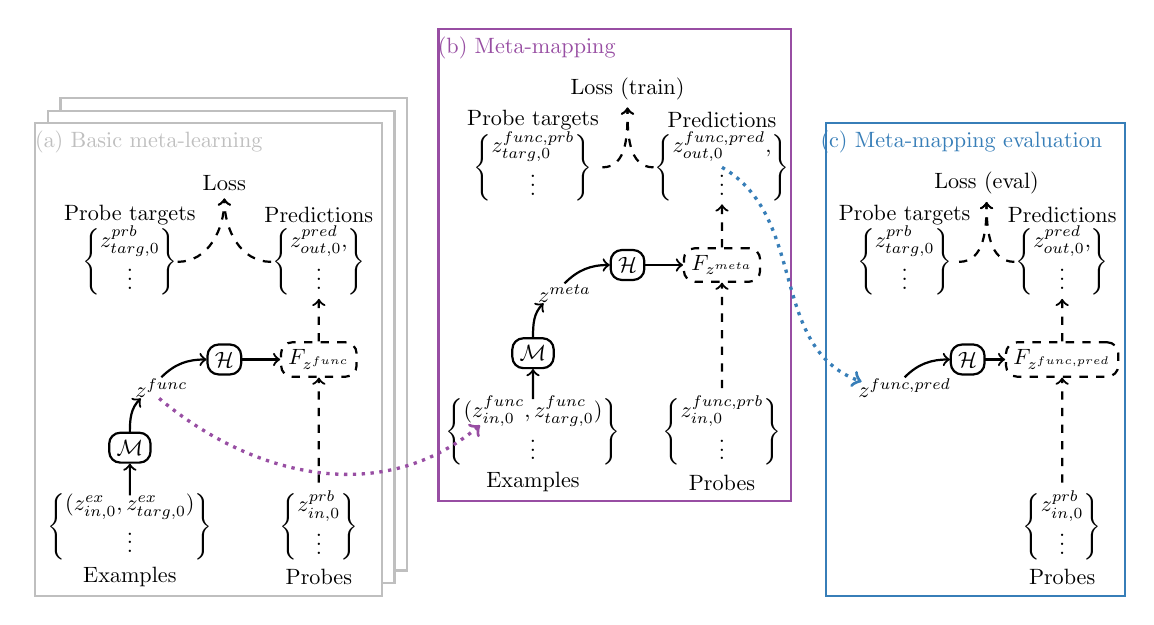
\begin{tikzpicture}[scale=0.8, every node/.style={scale=0.8}]
%% basic meta learning
\begin{scope}[shift={(0.4, 0.4)}]
\draw[boundingbox, fill=white] (-3, -4.3) rectangle (2.5, 3.2);
\end{scope}
\begin{scope}[shift={(0.2, 0.2)}]
\draw[boundingbox, fill=white] (-3, -4.3) rectangle (2.5, 3.2);
\end{scope}

\draw[boundingbox, fill=white] (-3, -4.3) rectangle (2.5, 3.2);
\node[lightgray] at (-1.2, 2.9) {(a) Basic meta-learning};
\node at (-1.5, -4) (examples) {Examples};
\node at (-1.5, -3.2) (D1) {
\(\left\{
\begin{matrix}
(z^{ex}_{in,0}, z^{ex}_{targ,0})\\
$\vdots$
\end{matrix}\right\}\)};

\node at (1.5, -4) (probes) {Probes};
\node at (1.5, -3.2) (D2) {
%\(z^{prb}_{in}\)};
\(\left\{
\begin{matrix}
z^{prb}_{in,0}\\
$\vdots$
\end{matrix}\right\}\)};

\node [block] at (-1.5, -1.95) (M) {\(\mathcal{M}\)};
\path [arrow] ([yshift=-5]D1.north) to (M);

\node at (-1, -1) (zfunc) {\(z^{func}\)};
\path [arrow, out=90, in=-135] (M.north) to ([xshift=6,yshift=3]zfunc.south west);

\node[block] at (0, -0.55) (H) {\(\mathcal{H}\)};
\path [arrow, out=45, in=180] ([yshift=-3]zfunc.north) to (H.west);

\node [block, dashed] at (1.5, -0.55) (F) {\(F_{z^{func}}\)};
\path[arrow] (H.east) to (F.west);

\path [arrow, dashed] (D2) to (F);

\node at (1.5, 1) (outputs) {
%\(z^{pred}_{out}\)};
\(\left\{
\begin{matrix}
z^{pred}_{out,0},\\
$\vdots$
\end{matrix}\right\}\)};
\node at (1.5, 1.75) (predictions) {Predictions};

\path [arrow, dashed] (F) to ([yshift=3]outputs.south);

\node at (-1.5, 1.75) (probetargs) {Probe targets};
\node at (-1.5, 1) (D2targs) {
%\(z^{prb}_{in}\)};
\(\left\{
\begin{matrix}
z^{prb}_{targ,0}\\
$\vdots$
\end{matrix}\right\}\)};

\node [align=center, text width=1.25 cm] at (0, 2.25) (dispatch) {\baselineskip=12pt Loss\par};

\path [arrow, dashed, out=180, in=-90] ([xshift=3]outputs.west) to (dispatch.south);

\path [arrow, dashed, out=0, in=-90] ([xshift=-3.5]D2targs.east) to (dispatch.south);



%% meta mapping
\begin{scope}[shift={(6.4, 1.5)}]
\draw[boundingbox, draw=bpurp, fill=white] (-3, -4.3) rectangle (2.6, 3.2);
\node[bpurp] at (-1.6, 2.9) {(b) Meta-mapping};
\node at (-1.5, -4) (metaexamples) {Examples};
\node at (-1.5, -3.2) (metaD1) {
\(\left\{
\begin{matrix}
(z^{func}_{in,0}, z^{func}_{targ,0})\\
$\vdots$
\end{matrix}\right\}\)};

\node at (1.5, -4) (metaprobes) {Probes};
\node at (1.5, -3.2) (metaD2) {
%\(z^{prb}_{in}\)};
\(\left\{
\begin{matrix}
z^{func,prb}_{in,0}\\
$\vdots$
\end{matrix}\right\}\)};

\node [block] at (-1.5, -1.95) (metaM) {\(\mathcal{M}\)};
\path [arrow] ([yshift=-5]metaD1.north) to (metaM);

\node at (-1, -1) (metazfunc) {\(z^{meta}\)};
\path [arrow, out=90, in=-135] (metaM.north) to ([xshift=6,yshift=3]metazfunc.south west);

\node[block] at (0, -0.55) (metaH) {\(\mathcal{H}\)};
\path [arrow, out=45, in=180] ([yshift=-3]metazfunc.north) to (metaH.west);

\node [block, dashed] at (1.5, -0.55) (metaF) {\(F_{z^{meta}}\)};
\path[arrow] (metaH.east) to (metaF.west);

\path [arrow, dashed] (metaD2) to (metaF);

\node at (1.5, 1) (metaoutputs) {
%\(z^{pred}_{out}\)};
\(\left\{
\begin{matrix}
z^{func,pred}_{out,0},\\
$\vdots$
\end{matrix}\right\}\)};
\node at (1.5, 1.75) (metapredictions) {Predictions};

\path [arrow, dashed] (metaF) to ([yshift=3]metaoutputs.south);

\node at (-1.5, 1.75) (metaprobetargs) {Probe targets};
\node at (-1.5, 1) (metaD2targs) {
%\(z^{prb}_{in}\)};
\(\left\{
\begin{matrix}
z^{func,prb}_{targ,0}\\
$\vdots$
\end{matrix}\right\}\)};

\node [align=center] at (0, 2.25) (metadispatch) {Loss (train)};

\path [arrow, dashed, out=180, in=-90] ([xshift=3]metaoutputs.west) to (metadispatch.south);

\path [arrow, dashed, out=0, in=-90] ([xshift=1]metaD2targs.east) to (metadispatch.south);


\end{scope}
\path [arrow, very thick, draw=bpurp, dotted, out=-40, in=-140] ([xshift=-1, yshift=3]zfunc.south) to ([xshift=19, yshift=3]metaD1.west);

%% evaluating meta mapping
\begin{scope}[shift={(11.8, 0)}]
\draw[boundingbox, draw=bblue, fill=white] (-2.25, -4.3) rectangle (2.5, 3.2);
\node[bblue] at (-0.1, 2.9) {(c) Meta-mapping evaluation};

\node at (1.5, -4) (metaevalprobes) {Probes};
\node at (1.5, -3.2) (metaevalD2) {
%\(z^{prb}_{in}\)};
\(\left\{
\begin{matrix}
z^{prb}_{in,0}\\
$\vdots$
\end{matrix}\right\}\)};

\node at (-1, -1) (metaevalzfunc) {\(z^{func,pred}\)};

\node[block] at (0, -0.55) (metaevalH) {\(\mathcal{H}\)};
\path [arrow, out=45, in=180] ([yshift=-3]metaevalzfunc.north) to (metaevalH.west);

\node [block, dashed] at (1.5, -0.55) (metaevalF) {\(F_{z^{func,pred}}\)};
\path[arrow] (metaevalH.east) to (metaevalF.west);

\path [arrow, dashed] (metaevalD2) to (metaevalF);

\node at (1.5, 1) (metaevaloutputs) {
%\(z^{pred}_{out}\)};
\(\left\{
\begin{matrix}
z^{pred}_{out,0},\\
$\vdots$
\end{matrix}\right\}\)};
\node at (1.5, 1.75) (metaevalpredictions) {Predictions};

\path [arrow, dashed] (metaevalF) to ([yshift=3]metaevaloutputs.south);

\node at (-1, 1.75) (metaevalprobetargs) {Probe targets};
\node at (-1, 1) (metaevalD2targs) {
%\(z^{prb}_{in}\)};
\(\left\{
\begin{matrix}
z^{prb}_{targ,0}\\
$\vdots$
\end{matrix}\right\}\)};

\node [align=center] at (0.3, 2.25) (metaevaldispatch) {Loss (eval)};

\path [arrow, dashed, out=180, in=-90] ([xshift=3]metaevaloutputs.west) to (metaevaldispatch.south);

\path [arrow, dashed, out=0, in=-90] ([xshift=-0.5]metaevalD2targs.east) to (metaevaldispatch.south);
\end{scope}
\path [arrow, very thick, draw=bblue, dotted, out=-30, in=160] (metaoutputs.center) to ([xshift=5, yshift=-5]metaevalzfunc.north west);
\end{tikzpicture}
\caption{The HoMM architecture allows for transformations at different levels of abstraction. (a) For basic meta-learning a dataset consisting of (input embedding, output embedding) tuples is processed by the meta-network \(\mathcal{M}\) to produce a function embedding \(z^{func}\), which is processed by the hyper network \(\mathcal{H}\) to parameterize a function \(F_{z^{func}}\), which attempts to compute the transformation on held-out probe inputs. However, our approach goes beyond basic meta-learning. The function embedding \(z^{func}\) can then be seen as a single input or output at the next level of abstraction, when the same networks \(\mathcal{M}\) and \(\mathcal{H}\) are used to transform function embeddings based on examples of a meta-mapping (b). To evaluate meta-mapping performance, a probe embedding of a held-out function is transformed by the architecture to yield a predicted embedding for the transformed task. The performance of this predicted embedding is evaluated by moving back down a level of abstraction and evaluating on the actual target task (c). Because the function embedding is predicted by a transformation rather than from examples, new tasks can be performed zero-shot. (\(M\) and \(H\) are learnable deep networks, and $F_{z}$ is a deep network parameterized by $\mathcal{H}$ conditioned on function embedding \(z\). Input and output encoders/decoders are omitted for simplicity. See the text and appendix \ref{app_model_details} for details.)} \label{architecture_inference_fig}
\end{figure}
\looseness=-1
More formally, we treat functions and data as entities of the same type. From this perspective, the data points that one function receives can themselves be functions\footnote{Indeed, any data point can be represented as a constant function that outputs the data point.}. The key insight is that then our architecture can transform data points\footnote{Where ``data'' is a quite flexible term. The approach is agnostic to whether the learning is supervised or reinforcement learning, whether inputs are images or natural language, etc.} to perform basic tasks (as is standard in machine learning), but it can also transform these task functions to adapt to new tasks. This is related to the concepts of homoiconicity, defined above, and higher-order functions. Under this perspective, basic tasks and meta-mappings from task to task are really the same type of problem. The functions at one level of abstraction (the basic tasks) become inputs and outputs for higher-level functions at the next level of abstraction (meta-mapping between tasks). \par
Specifically, we embed each input, target, or mapping into a shared representational space $Z$. This means that single data points are embedded in the same space as the representation of a function or an entire dataset. Inputs are embedded by a deep network $\mathcal{I}: \text{input} \rightarrow Z$. Model outputs are decoded from $Z$ by $\mathcal{O}: Z \rightarrow \text{output}$. Target outputs are encoded by $\mathcal{T}: \text{targets} \rightarrow Z$.\par
Given this, the task of mapping inputs to outputs can be framed as trying to find a transformation of the representational space that takes the (embedded) inputs from the training set to embeddings that will decode to the target outputs. These transformations are performed by a system with the following components (see fig. \ref{architecture_inference_fig}): $\mathcal{M}: \{(Z, Z), ...\} \rightarrow Z $ -- the meta network, which collapses a dataset of (input embedding, target embedding) pairs to produce a single function embedding. $\mathcal{H}: Z \rightarrow \text{parameters}$ -- the hyper network, which maps a function embedding to parameters. $F: Z \rightarrow Z$ -- the transformation, implemented by a deep network parameterized by $\mathcal{H}$. \par
\vspace{-0.5em}
\paragraph{Basic meta-learning:} To perform a basic task, input and target encoders ($\mathcal{I}$ and $\mathcal{T}$) are used to embed individual pairs from an example dataset \(D_1\), to form a dataset of example (input, output) tuples (fig. \ref{architecture_inference_fig}a). These examples are fed to $\mathcal{M}$, which produces a function embedding (via a deep neural network, with several layers of parallel processing across examples, followed by an element-wise max across examples, and several more layers). This function embedding is mapped through the hyper network $\mathcal{H}$ to parameterize $F$, and then $F$ is used to process a dataset of embedded probe inputs, and $\mathcal{O}$ to map the resultant embeddings to outputs. This system can be trained end-to-end on target outputs for the probes. Having two distinct datasets forces generalization at the meta-learning level, see appendix \ref{app_clarifying_holdouts}. See appendix \ref{app_model_details} for detailed architecture, and hyper-parameters. \par 
More explicitly, suppose we have a dataset of example input, target pairs ($D_1 = \{(x_0, y_0), ...\}$), and some input $x$ from a probe dataset $D_2$. The system would predict a corresponding output $\hat{y}$ as: 
\[\hat{y} = \mathcal{O}\left(F_{z^{func}}\left(\mathcal{I} \left(x\right)\right) \right)\]
where $F_{z^{func}}$ is the meta-learner's representation for the function underlying the examples in $D_1$:
\[F_{z^{func}} \text{ is parameterized by } \mathcal{H}\left(z^{func}\right), \text{ where } z^{func} = \mathcal{M}\left( \left\{\left(\mathcal{I}\left(x_0\right), \mathcal{T}\left(y_0\right) \right), ... \right\}\right)\]
Then, given some loss function $\mathfrak{L}(y, \hat{y})$ defined on a single target output $y$ and an actual model output $\hat{y}$, we define our total loss computed on the probe dataset $D_2$ as: 
\[\mathbb{E}_{(x, y)\in {D}_2} \left[ \mathfrak{L}\left(y, \mathcal{O}\left(F_{D_1}\left(\mathcal{I} \left(x\right)\right) \right)\right)\right]\]
The system can then be trained end-to-end on this loss to adjust the weights of \(\mathcal{T,H,M,O}\), and \(\mathcal{I}\).
\vspace{-0.25em}
\paragraph{Meta-mapping:} The fundamental insight of our paper is to show how basic tasks and meta-mappings can be treated homogenously, by allowing the network to transform its task representations like data (see fig. \ref{architecture_inference_fig}b,c). From the perspective of our architecture, learning a meta-mapping between tasks is exactly analogous to learning a basic task. Anything that is embedded in $Z$ can be transformed using the same system. Because tasks are embedded in $Z$ for basic meta-learning, this allows for meta-mappings using exactly the same $\mathcal{M}$ and $\mathcal{H}$ that we use for basic tasks. Just as we would take a set of paired embeddings of data points for a basic task, and use them to compute a function embedding for that task, we can take a set of paired function embeddings, and use them to create an embedding for the meta-mapping. We can then use this meta-mapping embedding to transform another task. We can thus behave zero-shot on a novel task based on its relationship to a prior task. \par
For example, suppose we have an embedding $z_{game1} \in Z$ for the task of playing some game. We can generate a meta-mapping embedding $z_{\text{meta}} \in Z$ from embeddings generated by the system when it is trying to win and lose various games: $z_{\text{meta}} = \mathcal{M}\left( \left\{\left((z_{game2},z_{game2,lose}\right), ... \right\}\right)$. We can generate a new task embedding $\hat{z}_{new} \in Z$:  
\[\hat{z}_{new} = F_{z_{\text{meta}}}(z_{game1}) \qquad \text{where } F_{z_{\text{meta}}} \text{ is parameterized by } \mathcal{H}\left(z_{\text{meta}}\right)\]
\looseness=-1
This $\hat{z}_{new}$ could be interpreted as the system's guess at a losing strategy for game 1. To train a meta-mapping, we minimize the $\ell_2$ loss in the latent space betwen this guessed embedding and the embedding of the target task. Whether or not we have such a target embedding, we can evaluate how well the system loses with this $\hat{z}_{new}$ strategy, by stepping back down a level of abstraction and actually having it play the game via this embedding (fig. \ref{architecture_inference_fig}c). This is how we evaluate meta-mapping performance -- evaluating the loss of transformed task embeddings on the respective target tasks. \par
Alternatively, we could map from language to a meta-mapping embedding, rather than inducing it from examples of the meta-mapping. This corresponds to the human ability to change behavior in response to instructions. The key feature of our architecture -- the fact that tasks, data, and language are all embedded in a shared space -- allows for substantial flexibility within a unified framework. Furthermore, our approach is parsimonious. Because it uses the same meta-learner for both basic tasks and meta-mappings, this increased flexibility does not require any added parameters.\footnote{At least in principle, in practice of course increasing network size might be more beneficial for HoMM architectures performing meta-mappings as well as basic tasks than for those performing only basic tasks.}  

%\subsection{Boolean functions}
%As a proof of concept, we first evaluated the system on a simple task of computing boolean functions on boolean inputs. Specifically, we can imagine mapping from binary-valued input vectors to a single binary output representing the evaluation of some logical proposition on the input. We train the system to figure out how to compute the predicate from seeing a subset of the (input, output) pairs. \par   
%We can then train the system to do various meta-mappings, for example identifying certain types of functions (like XOR) or negating predicates. \par
%
\section{Learning multivariate polynomials} \label{sec_poly}
\begin{figure}[t]
\centering
\begin{subfigure}[t]{0.5\textwidth}
\includegraphics[width=\textwidth]{figures/poly/basic_results.png}
\caption{The polynomials domain, section \ref{sec_poly}.}
\label{poly_basic_results}
\end{subfigure}%
\begin{subfigure}[t]{0.5\textwidth}
\includegraphics[width=\textwidth]{figures/basic_meta_learning.png}
\caption{The cards domain, section \ref{sec_cards}.}
\label{cards_basic_results}
\end{subfigure}%
\caption{The HoMM system succeeds at basic meta-learning, which is a necessary prerequisite for meta-mappings. (\subref{poly_basic_results}) The polynomials domain, section \ref{sec_poly}. The system successfully generalizes to held out polynomials. The solid line indicates optimal performance; the dashed line indicates untrained model performance. (\subref{cards_basic_results}) The card games domain, section \ref{sec_cards}. The system successfully generalizes to held out games, both when trained on a random sample of half the tasks, or when a targeted subset is held out. The gray dashed line indicates chance performance, while the solid lines are optimal performance. The orange dashed lines shows performance on held-out tasks of playing the strategy from the most correlated trained task. The fact that the system generally exceeds this difficult baseline shows a deeper form of generalization than just memorizing strategies and picking the closest. Error-bars throughout are bootstrap 95\%-confidence intervals, numerical values for plots can be found in appendix \ref{app_numerical_results}.}
\end{figure}

\begin{figure}[t]
\centering
\begin{subfigure}{0.5\textwidth}
\includegraphics[width=\textwidth]{figures/poly/meta_results.png}
\caption{The polynomials domain, section \ref{sec_poly}.}
\label{poly_meta_map_results_examples}
\end{subfigure}%
\begin{subfigure}{0.5\textwidth}
\includegraphics[width=\textwidth]{figures/meta_mapping.png}
\caption{The cards domain, section \ref{sec_cards}.}
\label{cards_meta_map_results_examples}
\end{subfigure}%
\caption{The HoMM architecture performs well at meta-mappings. (\subref{poly_meta_map_results_examples}) The system generalizes to apply learned meta-mappings to new polynomials, and even to apply unseen meta-mappings. The plots show the loss produced when evaluating the mapped embedding on the target task. For example, if the initial polynomial is $p(x) = x + 1$, and the meta-task is ``square,'' the loss would be evaluated by transforming the embedding of $p(x)$ and evaluating how well the mapped embedding regresses on to $p(x)^2 = x^2 + 2x + 1$. The results show that the system succeeds at applying meta-mappings it is trained on to held-out polynomials, as well as applying held-out meta-mappings to either trained or held-out polynomials. The solid line indicates optimal performance; the dashed line is untrained model performance.
(\subref{cards_meta_map_results_examples}) The system generalizes to meta-mapping new tasks in the cards domain. The system is trained to do the meta-mappings shown here on a subset of its basic tasks, and is able to generalize these mappings to perform novel tasks zero-shot. For example, for the ``losers'' mapping, the sytem is trained to map games to their losers variants. When given a held-out game, it is able to apply the mapping to guess how to play the losing variation. This plot shows the reward produced by taking the mapped embedding and playing the targeted game. The gray dashed line indicates random performance, while the colored dashed lines indicate performance if the system did not alter its behavior in response to the meta-mapping. The system generally exceeds these baselines, although the switch-suits baseline is more difficult with the targeted holdout. 
Error-bars are bootstrap 95\%-CIs.} 
\label{meta_map_results}
\end{figure}

As a proof of concept, we first evaluated the system on the task of learning polynomials of degree $\leq 2$ in 4 variables (i.e. the task was to regress functions of the form $p: \mathbb{R}^4 \rightarrow \mathbb{R}$ where $p \in \mathcal{P}_2 \left(\mathbb{R}\right)$, though the model was given no prior inductive bias toward polynomial forms). For example, if $p(w,x,y,z) = x$, the model might see examples like $(-1,1,1,1; 1)$ and $(0.7, 2.1, 1.3, -4; 2.1)$, and be evaluated on its output for points like $(-1, -1.3, 0.5, 0.3)$. This yields an infinite family of base-level tasks (the vector space of all such polynomials), as well as many families of meta-mappings over tasks (for example, multiplying polynomials by a constant, squaring them, or permuting their input variables). This allows us to not only examine the ability of the system to learn to learn polynomials from data, but also to adapt its learned representations in accordance with these meta-tasks. Details of the architecture and training can be found in appendix \ref{app_detailed_methods}.\par
\vspace{-0.7em}
\paragraph{Basic meta-learning:} First, we show that the system is able to achieve the basic goal of learning a held-out polynomial from a few data points in fig. \ref{poly_basic_results} (with good sample-efficiency, see supp. fig. \ref{supp_poly_sweep_results}). \par 
\vspace{-0.7em}
\paragraph{Meta-mapping (task $\rightarrow$ task):} Furthermore, the system is able to perform meta-mappings over polynomials in order to flexibly reconfigure its behavior (fig. \ref{poly_meta_map_results_examples}). We train the system to perform a variety of mappings, for example switch the first two inputs of the polynomial, add 3 to the polynomial, or square the polynomial. We then test its ability to generalize to held-out mappings from examples, for example a held-out input permutation, or an unseen additive shift. The system is both able to apply learned meta-mappings to held-out polynomials, and to apply held-out meta-mappings it has not been trained on, simply by seeing examples of the mapping. \par 

\section{A stochastic learning setting: simple card games}\label{sec_cards}
%\vspace{-0.5em} % section
We next explored the setting of simple card games, where the agent is dealt a hand and must bet. There are three possible bets (including ``don't bet''), and depending on the opponent's hand the agent either wins or loses the amount bet. This task doesn't require long term planning, but does incorporate some aspects of reinforcement learning, namely stochastic feedback on only the action chosen. We considered five games that are simplified analogs of various real card games (see Appendix \ref{meth_data_cards}). We also considered several binary options that could be applied to the games, including trying to lose instead of trying to win, or switching which suit was more valuable. These are challenging manipulations, for instance trying to lose requires completely inverting a learned $Q$-function. \par
%% Can cut The hand is explicitly ..., maybe some other stuff
In order to adapt the HoMM architecture, we made a very simple change. Instead of providing the system with (input, target) tuples to embed, we provided it with (state, action, reward) tuples, and trained it to predict rewards for each bet in each state. (A full RL framework is not strictly necessary here because there is no temporal aspect to the tasks; however, because the outcome is only observed for the action you take, it is not a standard supervised task.) The hand is explicitly provided to the network for each example, but which game is being played is implicitly captured in the training examples, without any explicit cues. That is, the system must learn to play directly from seeing a set of (state, action, reward) tuples which implicitly capture the structure and stochasticity of the game. We also trained the system to make meta-mappings, for example switching from trying to win a game to trying to lose. Details of the architecture and training can be found in appendix \ref{app_detailed_methods}. \par
%\vspace{-0.7em}
\paragraph{Basic meta-learning:} First, we show that the system is able to play a held-out game from examples in fig. \ref{cards_basic_results}. We compare two different hold-out sets: 1) train on half the tasks at random, or 2) specifically hold out all the ``losers'' variations of the ``straight flush'' game. In either of these cases, the meta-learning system achieves well above chance performance (0) at the held out tasks, although it is slightly worse at generalizing to the targeted hold out, despite having more training tasks in that case. Note that the sample complexity in terms of number of trained tasks is not that high, even training on 20 randomly selected tasks leads to good generalization to the held-out tasks. Furthermore, the task embeddings generated by the system are semantically organized, see appendix \ref{app_cards_tsne}. \par
%\vspace{-0.7em}
\paragraph{Meta-mapping (task $\rightarrow$ task):} Furthermore, the system is able to perform meta-mappings (mappings over tasks) in order to flexibly reconfigure its behavior. For example, if the system is trained to map games to their losers variations, it can generalize this mapping to a game it has not been trained to map, even if the source or target of that mapping is held out from training. In fig. \ref{cards_meta_map_results_examples} we demonstrate this by taking the mapped embedding and evaluating the reward received by playing the targeted game with it. This task is more difficult than simply learning to play a held out game from examples, because the system will actually receive no examples of the target game (when it is held out). Furthermore, in the case of the losers mapping, leaving the strategy unchanged would produce a large negative reward, and chance performance would produce 0 reward, so the results are quite good. \par
%\vspace{-0.5em}
\section{An extension via language}
%\vspace{-0.5em} % section
\begin{figure}
\centering
\begin{subfigure}{0.5\textwidth}
\includegraphics[width=\textwidth]{figures/poly/language_meta_results.png}
\caption{From language input.}
\label{poly_meta_map_results_language}
\end{subfigure}%
\begin{subfigure}{0.5\textwidth}
\includegraphics[width=\textwidth]{figures/language_meta_mapping.png}
\caption{From language input.}
\label{cards_meta_map_results_language}
\end{subfigure}
\caption{The HoMM system can perform meta-mappings from language cues rather than meta-mapping examples. Compare to fig. \ref{meta_map_results}, which shows the same results when using examples instead of language. (\subref{poly_meta_map_results_language}) In the polynomials domain, language cues still lead to good performance, even on held-out tasks or held-out meta-mappings, although examples perform slightly better (fig. \ref{poly_meta_map_results_examples}). (\subref{cards_meta_map_results_language}) Similarly, in the cards domain, language cues perform well. Error-bars are bootstrap 95\%-CIs.}
\label{language_meta_map_results}
\end{figure}
Language is fundamental to human flexibility. Often the examples of the meta-mapping are implicit in prior knowledge about the world that is cued by language. For example, ``try to lose at go'' does not give explicit examples of the ``lose'' meta-mapping, but rather relies on prior knowledge of what losing means. This is a much more efficient way to cue a known meta-mapping. In order to replicate this, we trained the HoMM system with both meta-mappings based on examples, and meta-mappings based on language. In the language-based meta-mappings, a language input identifying the meta-mapping (but not the basic task to apply it to) is encoded by a language encoder, and then provided as the input to $\mathcal{H}$ (instead of an output from $\mathcal{M}$). The meta-mapping then proceeds as normal --- $\mathcal{H}$ parameterizes $F$, which is used to transform the embedding of the input task to produce an embedding for the target. \par
This language-cued meta-mapping approach also yields good performance (fig. \ref{language_meta_map_results}). However, examples of the meta-mapping are slightly better, especially for meta-mappings not seen during training, presumably because examples provide a richer description. In Appendix \ref{app_why_meta_mapping} we show that using language to specify a meta-mapping performs better than using language to directly specify the target task, presumably by leveraging the richer task representation of the task embedding. \par

%\vspace{-0.5em}
\section{Discussion} \label{sec_discussion}
%\vspace{-0.5em} % section
\paragraph{Related work:} Our work is an extrapolation from the rapidly-growing literature on meta-learning \citep[e.g.][]{Vinyals2016, Santoro2016, Finn2017a, Finn2018, Stadie2018, Botvinick2019}. It is also related to the literature on continual learning, or more generally tools for avoiding catastrophic interference based on changes to the architecture \citep[e.g.][]{Fernando2017, Rusu2016}, loss \citep[e.g.][]{Kirkpatrick2016, Zenke2017, Aljundi2019}, or external memory \citep[e.g.][]{Sprechmann2018}. We also connect to a different perspective on continual learning in appendix \ref{app_continual}. Recent work has also begun to blur the separation between these approaches, for example by meta-learning in an online setting \citep{Finn2019}. Our work is specifically inspired by the algorithms that attempt to have the system learn to adapt to a new task via activations rather than weight updates, either from examples \citep[e.g.][]{Wang2016a, Duan2016}, or a task input \citep[e.g.][]{Borsa2019}. \par
Our architecture builds directly off of prior work on HyperNetworks \citep{Ha2016} -- networks which parameterize other networks -- and other recent applications thereof, such as guessing parameters for a model to accelerate model search \citep[e.g.][]{Brock2018a, Zhang2019}, and meta-learning \citep[e.g.]{Li2019a, Rusu2019}. Our work is also related to the longer history of work on different time-scales of weight adaptation \citep{Hinton1982, Kumaran2016} that has more recently been applied to meta-learning contexts \citep[e.g.][]{Ba2016, Munkhdalai2017, Garnelo2018} and continual learning \citep[e.g.]{Hu2019}. It is more abstractly related to work on learning to propose architectures \citep[e.g.][]{Zoph2016, Cao2019}, and to models that learn to select and compose skills to apply to new tasks \citep[e.g.][]{Andreas, Andreas2016, Tessler2016, Reed2015, Chang2019a}. In particular, some of the work in domains like visual question answering has explicitly explored the idea of building a classifier conditioned on a question \citep{Andreas, Andreasa}, which is related to one of the possible computational paths through our architecture. Work in model-based reinforcement learning has also partly addressed how to transfer knowledge between different reward functions \citep[e.g.][]{Laroche2017}; our approach is more general. Indeed, our insights could be combined with model-based approaches, for example our approach could be used to adapt a task embedding, which would then be used by a learned planning model.\par 
There has also been other recent interest in task (or function) embeddings. Achille et al. \citep{Achille2019} recently proposed computing embeddings for visual tasks from the Fisher information of the parameters in a model partly tuned on the task. They show that this captures some interesting properties of the tasks, including some types of semantic relationships, and can help identify models that can perform well on a task. Rusu and colleagues recently suggested a similar meta-learning framework where latent codes are computed for a task which can be decoded to a distribution over parameters \citep{Rusu2019}. Other recent work has tried to learn representations for skills \citep[e.g.][]{Eysenbach2019} or tasks \citep[e.g.]{Hsu2019} for exploration and representation learning. Our perspective can be seen as a generalization of these that allows for remapping of behavior via meta-tasks. To the best of our knowledge none of the prior work has explored zero-shot performance of a task via meta-mappings. \par
% \vspace{-1em}
\paragraph{Future Directions:} We think that the general perspective of considering meta-mappings will yield many fruitful future directions. We hope that our work will inspire more exploration of behavioral adaptation, in areas beyond the simple domains we considered here. To this end, we suggest the creation of meta-learning datasets which include information not only about tasks, but about the relationships between them. For example, reinforcement learning tasks which involve executing instructions \citep[e.g.][]{Hermann2017, Co-Reyes2019} can be usefully interpreted from this perspective. Furthermore, we think our work provides a novel perspective on the types of flexibility that human intelligence exhibits, and thus hope that it may have implications for cognitive science. \par 
We do not necessarily believe that the particular architecture we have suggested is the best architecture for addressing these problems, although it has a number of desirable characteristics. However, the modularization of the architecture makes it easy to modify. (We compare some variations in appendix \ref{app_lesion_results}.) For example, although we only considered task networks $F$ that are feed-forward and of a fixed depth, this could be replaced with a recurrent architecture to allow more adaptive computation, or even a more complex architecture \citep[e.g.][]{Reed2015, Graves2016}. Our work also opens the possibility of doing unsupervised learning over function representations for further learning, which relates to long-standing ideas in cognitive science about how humans represent knowledge \citep{Clark1993}. \par 
%\vspace{-1em}
%\paragraph{Conclusions:}
\section{Conclusions}
%\vspace{-0.5em} % section
\looseness=-1
We've highlighted a new type of flexibility in the form of meta-mapping between tasks. Meta-mapping can produce zero-shot performance on novel tasks, based on their relationship to old tasks. However, achieving this flexibility is difficult in architectures that separate computation from the knowledge of what is being computed. To address this, our Homoiconic Meta-Mapping (HoMM) approach explicitly represents tasks by function embeddings, and derives the computation from these embeddings via a HyperNetwork. This allows for our key insight: by embedding tasks and individual data points in a shared latent space, the same meta-learning architecture can be used both to transform data for basic tasks, and to transformat task embeddings to adapt to task variations. This approach is parsiomious, because it uses the same networks for basic- and meta-mappings. Perhaps because of this, the requisite meta-task sample complexity is small; we showed generalization to unseen meta-mappings after training on only 20 meta-mappings. That is, we are able to achieve zero-shot performance on a novel task based on a held-out relationship between tasks. This is a step closer to human-level flexibility.\par
We see our proposal as a logical progression from the fundamental idea of meta-learning -- that there is a continuum between data and tasks. This naturally leads to the idea of manipulating task representations just like we manipulate data. We've shown that this approach yields considerable flexibility, most importantly the meta-mapping ability to adapt zero-shot to a new task. We hope that these results will lead to the development of more powerful and flexible deep-learning models. \par
%\subsubsection*{Acknowledgements}
%We would like to acknowledge Noah Goodman, Surya Ganguli, Katherine Hermann, Erin Bennett, and Arianna Yuan for stimulating questions and suggestions on this project.

\bibliographystyle{apalike}
\bibliography{arrr}

\newpage
% comment the following to compile without appendix but with references
\include{homoiconic_meta_mapping_appendix}

\end{document}
